\section{Test}
In questa sezione vengono descritte le attività di testing svolte durante questa iterazione, con l’obiettivo di verificare la correttezza, l’affidabilità e la stabilità delle nuove funzionalità introdotte. I test sono stati condotti sia a livello di singoli componenti, per validare la logica di business, sia a livello di integrazione, per assicurare il corretto funzionamento delle API esposte e la comunicazione tra frontend e backend. Particolare attenzione è stata dedicata alla verifica degli endpoint relativi alla gestione dei viaggi e delle nuove funzionalità introdotte, includendo operazioni di visualizzazione del catalogo pubblico, consultazione dello storico, applicazione dei filtri di ricerca, gestione dei percorsi preferiti e aggiornamento dello stato dei viaggi come completati. Sono state inoltre testate le funzionalità di creazione di itinerari casuali e di modifica delle tappe, comprensive del ricalcolo del percorso ottimizzato tramite il motore TSP.
\subsection{Test: CodeMR}
L'analisi statica del codice per la seconda iterazione è stata condotta tramite CodeMR. Rispetto all'iterazione precedente, le metriche riflettono la naturale espansione del sistema: le linee di codice totali sono aumentate e il numero di classi anche. Nonostante l'introduzione di numerose funzionalità (catalogo pubblico, storico, filtri e percorsi casuali), l'architettura mantiene un livello di qualità elevato, registrando zero classi "altamente problematiche" e solo tre classi "problematiche".
Di seguito vengono analizzate le tre metriche principali: Complessità, Accoppiamento e Mancanza di Coesione.

\begin{figure}
    \centering
    \begin{minipage}{0.30\textwidth}
        \centering
        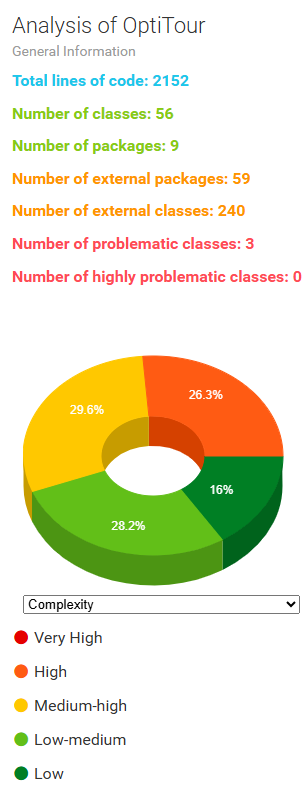
\includegraphics[width=\textwidth]{Iterazione2/Diagrammi/codeMR/complexityIT2.png}
        \caption{Complessità.}
        \label{fig:codemr_complexity}
    \end{minipage}\hfill
    \begin{minipage}{0.30\textwidth}
        \centering
        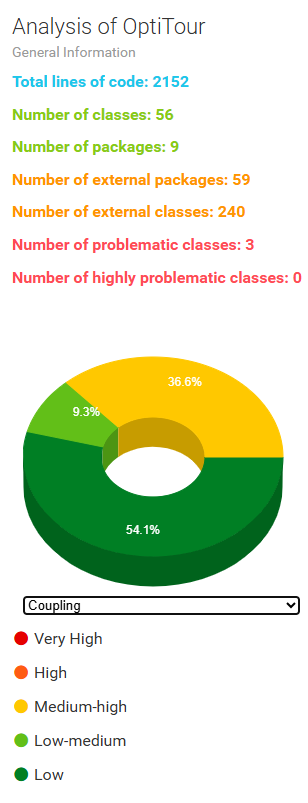
\includegraphics[width=\textwidth]{Iterazione2/Diagrammi/codeMR/CouplingIT2.png}
        \caption{Accoppiamento.}
        \label{fig:codemr_coupling}
    \end{minipage}\hfill
    \begin{minipage}{0.30\textwidth}
        \centering
        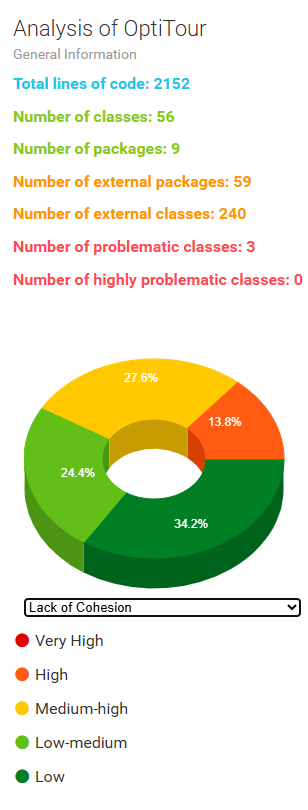
\includegraphics[width=\textwidth]{Iterazione2/Diagrammi/codeMR/CoesioneIT2.png}
        \caption{Lack of Cohesion.}
        \label{fig:codemr_cohesion}
    \end{minipage}
\end{figure}

\begin{itemize}
    \item \textbf{Complessità:} L'aggiunta di logiche avanzate ha comportato un fisiologico aumento della complessità in alcune classi. Tuttavia, la maggior parte del sistema si mantiene su livelli bassi o medio-bassi.
    \item \textbf{Accoppiamento:} I risultati confermano l'efficacia dell'architettura a livelli (MVC) e dell'uso delle interfacce. Oltre il 54\% delle classi ha un livello di accoppiamento "Basso" e non si registrano classi nella fascia "Alta" o "Molto Alta".
    \item \textbf{Coesione:} La distribuzione rimane bilanciata. Una buona porzione del sistema mostra un'alta coesione (indicata dai valori bassi/verdi di "Lack of Cohesion"), sinonimo di classi robuste, con responsabilità singole ben definite e facili da manutenere.
\end{itemize}

\subsubsection*{Analisi delle Classi Complesse e Struttura dei Package}
L'analisi di dettaglio ha evidenziato che la classe con il maggior grado di complessità è il \texttt{TripService} (\autoref{fig:classe_complex}). Questo risultato è ampiamente giustificato: come dimostrato anche nei test JUnit, il \texttt{TripService} funge da gestore centrale della logica di business, gestendo le validazioni, la sicurezza, la storicizzazione, il ricalcolo del TSP e l'integrazione con i database per tutto il ciclo di vita dei viaggi. L'accoppiamento e la mancanza di coesione per questa classe rimangono comunque nella fascia media.
\begin{figure}
    \centering
    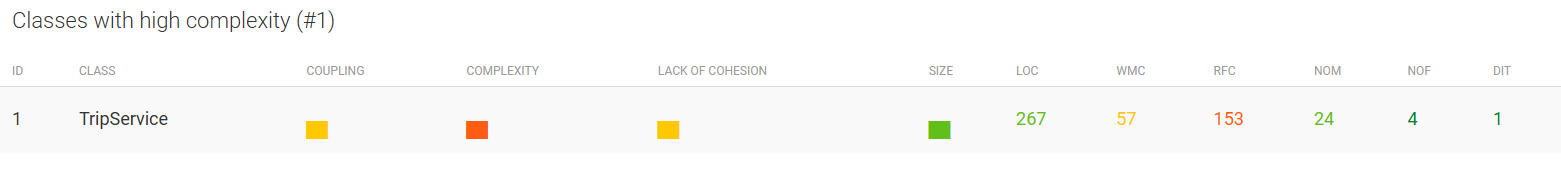
\includegraphics[width=0.7\textwidth]{Iterazione2/Diagrammi/codeMR/ClasseAltaComplex.png}
    \caption{Dettaglio della classe TripService, identificata con complessità alta.}
    \label{fig:classe_complex}
\end{figure}
Infine, la visualizzazione della metrica strutturale per package (\autoref{fig:struttura_codemr}) conferma che i pesi maggiori in termini di dimensioni e complessità risiedono nei layer \texttt{service}, \texttt{model} e \texttt{dto}. Al contrario, il layer \texttt{controller} mantiene dimensioni più contenute, limitandosi correttamente a intercettare e instradare le chiamate esterne senza inglobare logica applicativa.
\begin{figure}
    \centering
    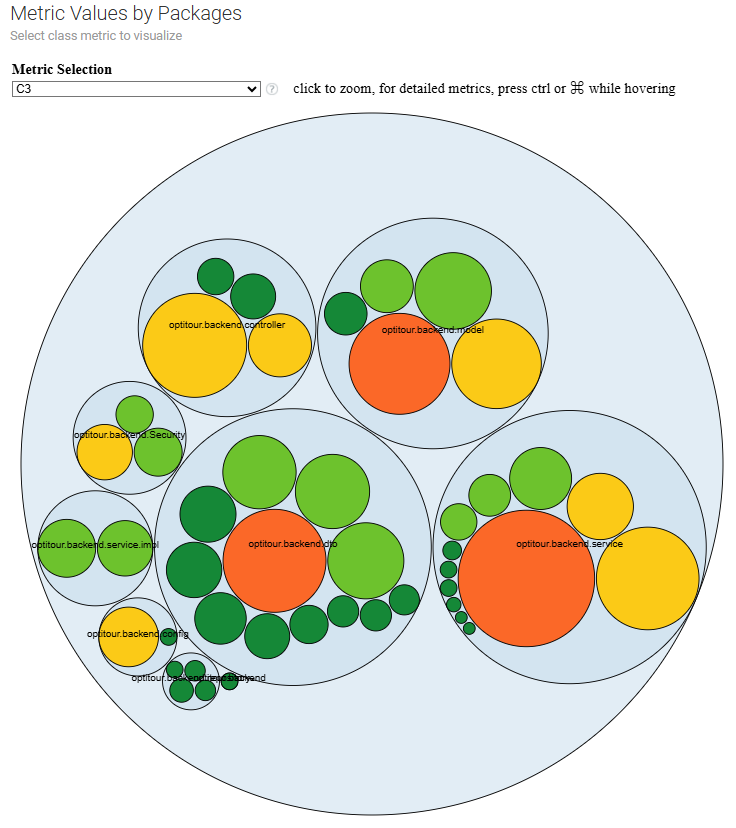
\includegraphics[width=0.7\textwidth]{Iterazione2/Diagrammi/codeMR/strutturaIT2.png}
    \caption{Distribuzione delle metriche all'interno dei package architetturali.}
    \label{fig:struttura_codemr}
\end{figure}

\newpage
\subsection{Test: Junit}
Questa sezione è dedicata ai test eseguiti con JUnit. La copertura dei test riguardanti l'autenticazione base, la gestione degli utenti, l'integrazione con le API dei monumenti e l'algoritmo centrale del TSP è rimasta inalterata rispetto all'Iterazione 1, risultando quindi già del tutto validata.

\subsubsection*{1. Sicurezza e Validazione Token}
 Sono stati aggiunti test specifici per il livello di sicurezza, questi nuovi moduli verificano la corretta autorizzazione delle richieste HTTP tramite i filtri JWT, gestendo casi limite come l'uso di token malformati, revocati o scaduti (\autoref{fig:auth_test} e  \autoref{fig:token_test}), oltre a validare la logica di estrazione dei dettagli utente dal database ( \autoref{fig:custom_detail_test}).

\begin{figure}[H]
    \centering
    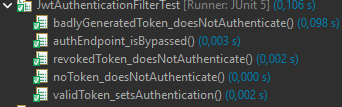
\includegraphics[width=0.7\textwidth]{Iterazione2/Diagrammi/test/AuthTest.png}
    \caption{Test del filtro di autenticazione JWT e gestione dei token.}
    \label{fig:auth_test}
\end{figure}
\begin{figure}[H]
    \centering
    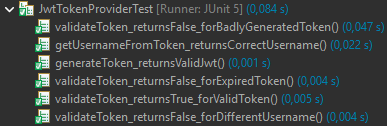
\includegraphics[width=0.7\textwidth]{Iterazione2/Diagrammi/test/TokenTest.png}
    \caption{Validazione del Provider JWT.}
    \label{fig:token_test}
\end{figure}
\begin{figure}[H]
    \centering
    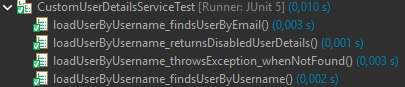
\includegraphics[width=0.7\textwidth]{Iterazione2/Diagrammi/test/CustomDetailService.png}
    \caption{Test del Custom User Details Service.}
    \label{fig:custom_detail_test}
\end{figure}


\subsubsection*{2. Gestione Viaggi (TripService e TripController)}
Il cuore del lavoro di testing di questa iterazione si è concentrato sull'espansione dei controller e dei service legati ai viaggi, che ora coprono un vasto ventaglio di nuovi casi d'uso. Come viene mostrato in \autoref{fig:trip_controller_test}, i test a livello di Controller validano l'esposizione delle nuove API per il recupero dei viaggi pubblici (catalogo), l'applicazione di filtri case-insensitive per città e la corretta gestione degli stati del viaggio (salvataggio nei preferiti, completamento, ripristino).

\begin{figure}
    \centering
    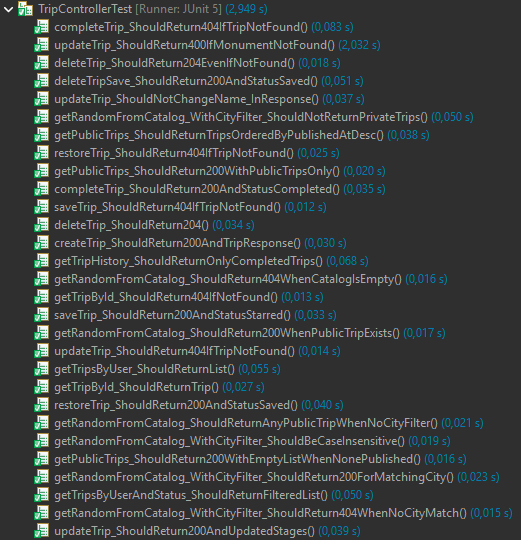
\includegraphics[width=0.9\textwidth]{Iterazione2/Diagrammi/test/TripControllerTest.png}
    \caption{Espansione dei test sugli endpoint del TripController.}
    \label{fig:trip_controller_test}
\end{figure}

A livello di logica di business, il \texttt{TripServiceTest} (\autoref{fig:trip_service_test}) è stato arricchito per validare rigorosamente le regole applicative. I test assicurano che:
\begin{itemize}
    \item La generazione casuale dei viaggi rispetti i vincoli imposti.
    \item Vengano applicati rigorosi controlli di sicurezza (es. eccezione 403 Forbidden se un utente tenta di modificare o pubblicare un viaggio non suo).
    \item I flussi di pubblicazione (IsPublic) e la storicizzazione funzionino in stretta sinergia con il database.
\end{itemize}

\begin{figure}
    \centering
    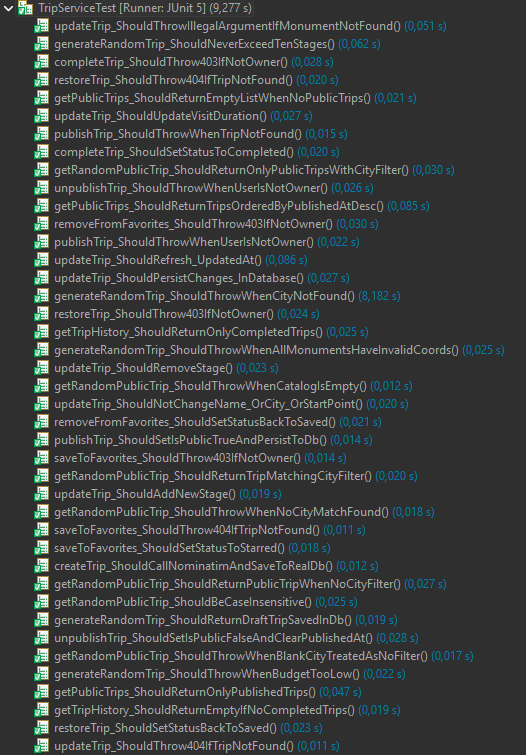
\includegraphics[width=0.8\textwidth]{Iterazione2/Diagrammi/test/TripServiceTest.png}
    \caption{Espansione dei test della logica di business nel TripServiceTest.}
    \label{fig:trip_service_test}
\end{figure}

\newpage
\subsection{API Esposte}

In questa sezione vengono descritte le principali API esposte dal backend tramite i controller di Spring Boot, necessarie per supportare i casi d’uso sviluppati e testate tramite Postman.

\begin{enumerate}

\item \textbf{Gestione Viaggi}

\textbf{Aggiornamento di un Viaggio}

\begin{itemize}
    \item \textbf{Endpoint:} PUT /api/trips/\{id\}

    \item \textbf{Descrizione:} Permette di aggiornare un viaggio esistente modificandone le informazioni principali, come la durata per ciascuna tappa, l’aggiunta e la rimozione di tappe con le relative tempistiche. 
    I dettagli della richiesta e della risposta sono illustrati in \autoref{fig:updateTripRequest} e Figura \autoref{fig:updateTripResponse}.

    \item \textbf{Parametri:}
    \begin{itemize}
        \item \{id\} (string) - ID del viaggio da aggiornare.
    \end{itemize}

    \item \textbf{Payload:}
    \begin{itemize}
        \item name (string) - Nome del viaggio.
        \item city (string) - Città del viaggio.
        \item startPoint (string) - Punto di partenza.
        \item stages (array) - Lista aggiornata delle tappe del viaggio.
    \end{itemize}

\end{itemize}

\end{enumerate}

\begin{figure}[H]
    \centering
    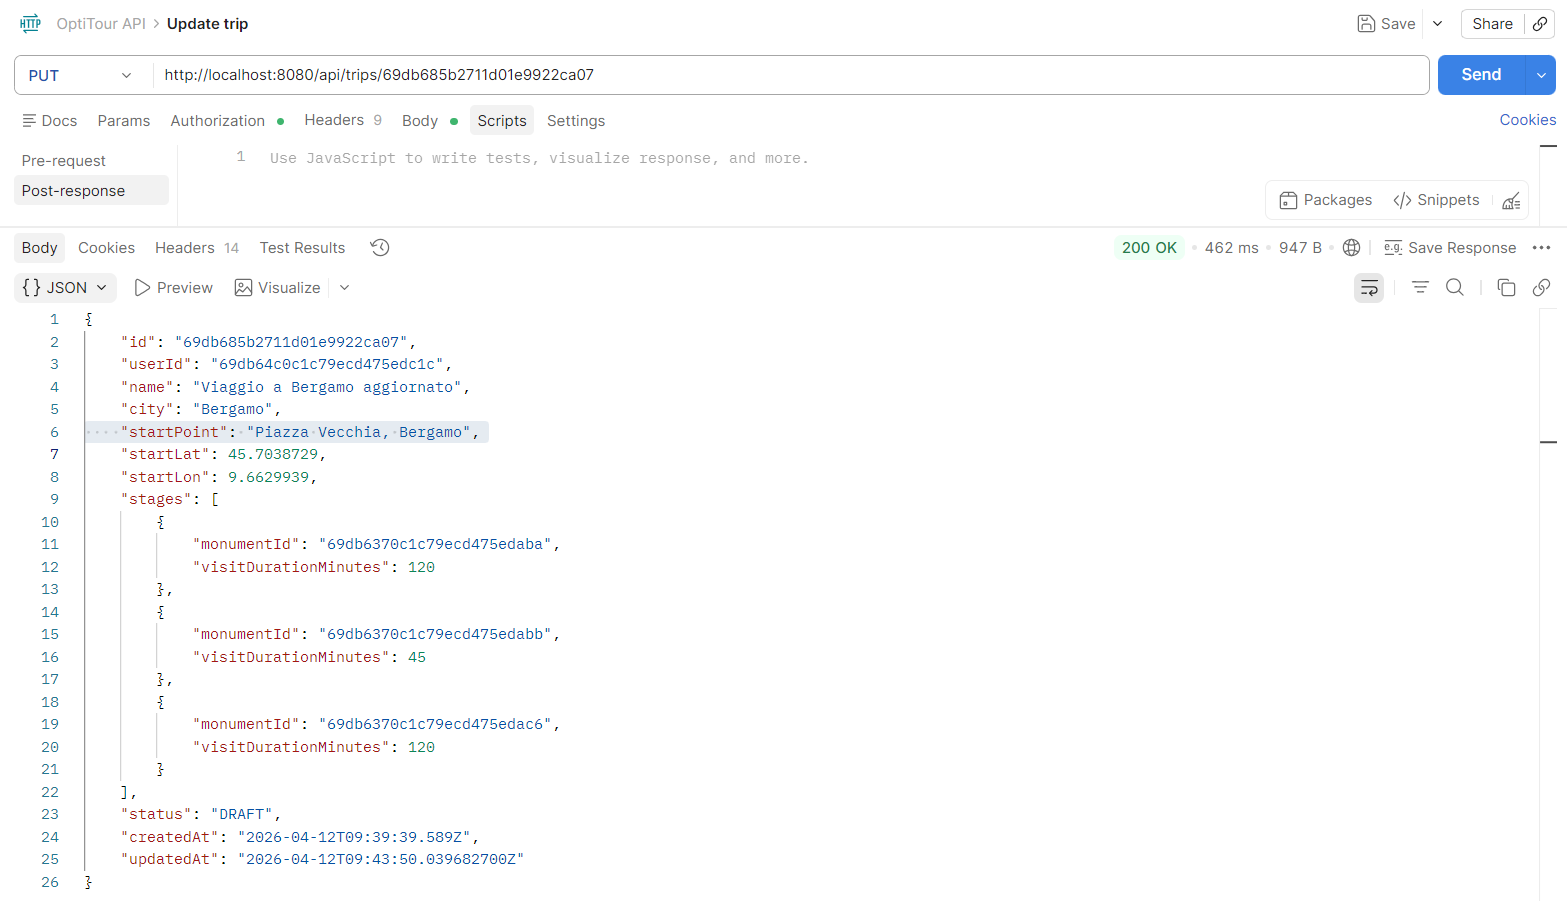
\includegraphics[width=0.8\textwidth]{Iterazione2/Diagrammi/API/updateTripApi.png}
    \caption{Test su Postman: Payload di richiesta per l’aggiornamento di un viaggio.}
    \label{fig:updateTripRequest}
\end{figure}

\begin{figure}[H]
    \centering
    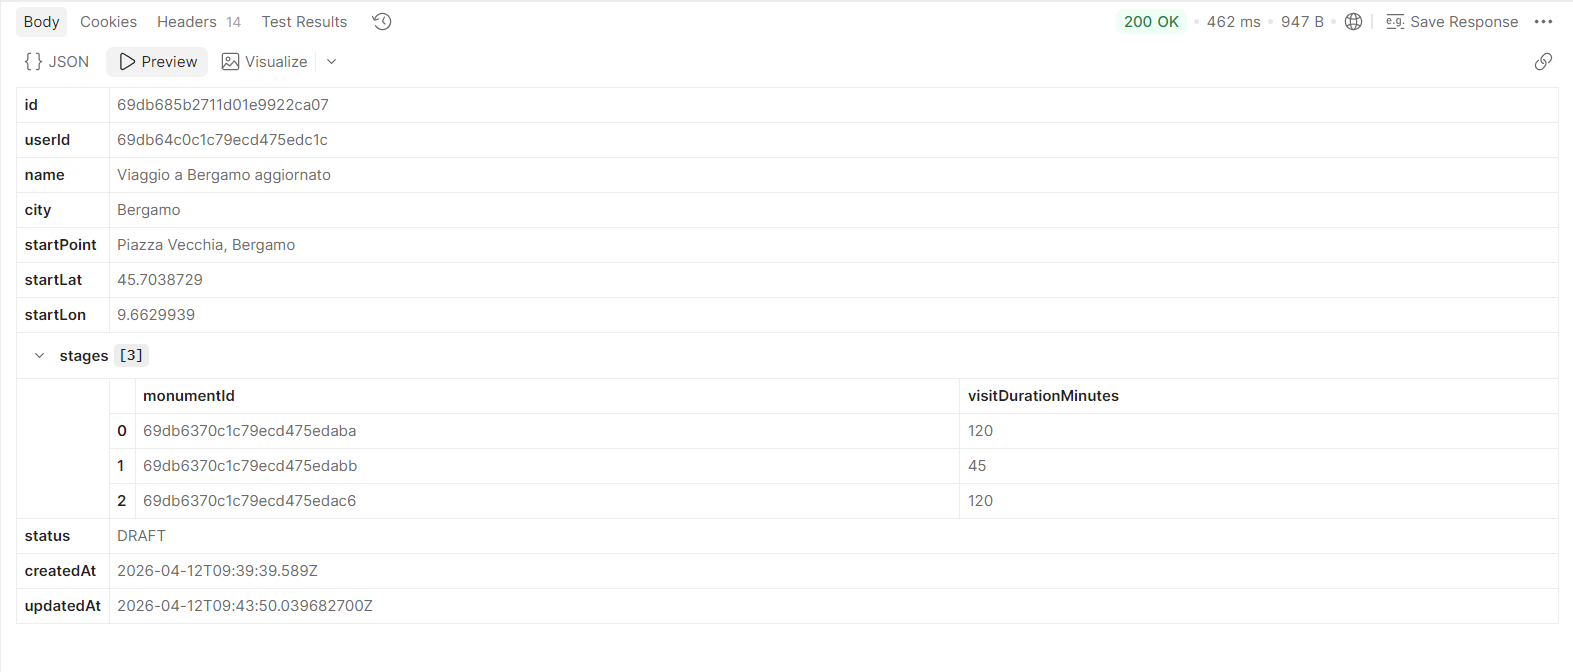
\includegraphics[width=0.8\textwidth]{Iterazione2/Diagrammi/API/updateTripApiResponse.png}
    \caption{Test su Postman: Risposta del server dopo l’aggiornamento del viaggio.}
    \label{fig:updateTripResponse}
\end{figure}

